\chapter{Event Selection}
\label{chap:Selection}

Events are required to contain exactly three \emph{tight} leptons described in \autoref{sec:Leptons}. Furthermore, events are selected with \ac{HLT} triggers discussed in \autoref{sec:Triggers}. Events with different lepton flavor composites are further categorized into three exclusive channels: eee, $\mmm$, $\emul$. In all three channels, the sum of the electric charges of the selected leptons is required to be 1 or -1. The leading leptons in all selected events are required to be matched with trigger objects within $\mathrm{\Delta} R~<$ 0.2. Within each channel, different regions are defined to further understand signal and background.

$\emul$ is the channel where close to 100\% of the simulated signal events reside. This channel is divided into signal-enriched \acp{SR} and signal-depleted \acp{VR}, which are discussed in \autoref{sec:SR} and \autoref{sec:VR}, respectively. Due to the lack of different flavors, the eee and $\mmm$ channels are signal-depleted by definition. Therefore, events found in these two channels are only used to study background processes, which are discussed in \autoref{sec:VR}. The kinematic reconstruction of heavy particles, such as the top quark, is described in \autoref{sec:Kin}.
%%%%%%%%%%%%%%%%%%%%%%%%%%%%%%%%%%%%%%%%%%%%%%%%%%%%%%%%%%%%%
%%%%%%%%%%%%%%%%%%%%%%%%%%%%%%%%%%%%%%%%%%%%%%%%%%%%%%%%%%%%%
\section{Signal Region}
\label{sec:SR}

The core feature of the signal events is the presence of the ``LFV e$\upmu$'' pair, which consists of a pair of \ac{OSDF} leptons. It is guaranteed that there is at least one \ac{OSDF} pair in all events residing in $\emul$ channel due to the requirement on electric charges. The \ac{OSDF} pair is immediately labeled as the LFV e$\upmu$ pair if it is only possible to reconstruct one \ac{OSDF} pair. In events where a pair of \ac{SSSF} leptons are present, a kinematic reconstruction is used to determine which one of two leptons form the LFV e$\upmu$ pair with the third lepton, which is detailed in \autoref{sec:Kin}. Leptons that form the LFV e$\upmu$ pair are referred to as the LFV electron or muon as it is assumed that they originate from the \ac{CLFV} interaction. Based on the event topology of the signal process, further selection criteria are applied to define the \ac{SR}. These selection criteria help achieve an optimal signal-to-background ratio by removing the majority of the background events present in $\emul$ channel. 

At the tree-level, signal events are expected to contain one or two jets, which motivates a requirement of at least one jet in \ac{SR}. Furthermore, it is required that there is no more than one b-tagged jet to suppress the contribution from $\ttbar$ events. Another prominent background is \ac{DY} production that features an \ac{OSSF} pair. To suppress \ac{DY} processes in \ac{SR}, events that contain an \ac{OSSF} lepton pair with an invariant mass between 50 GeV and 106 GeV are removed. The lower bound of this veto is lower than the typical value (e.g. 75 GeV) because the mass range between 50 GeV and 75 GeV has very few signal events and is dominated by \emph{nonprompt} background from photon conversion. Additionally, a modest threshold of 20 GeV is applied to \ac{MET} due to the presence of neutrinos in the signal events.

Distributions of the LFV e$\upmu$ mass and the Z boson mass are shown in Figure~\ref{fig:SR}. All backgrounds in Figure~\ref{fig:SR} are estimated using \ac{MC} simulation even though the strategy is to use a data-driven method to estimate the \emph{nonprompt} background. This serves as a preliminary check to understand the components of different backgrounds in \ac{SR}. Distributions of more variables in \ac{SR} are included in \autoref{chap:SRMC}.

\begin{figure}[tbh!]
 \begin{center}
 \begin{tabular}{cc}
 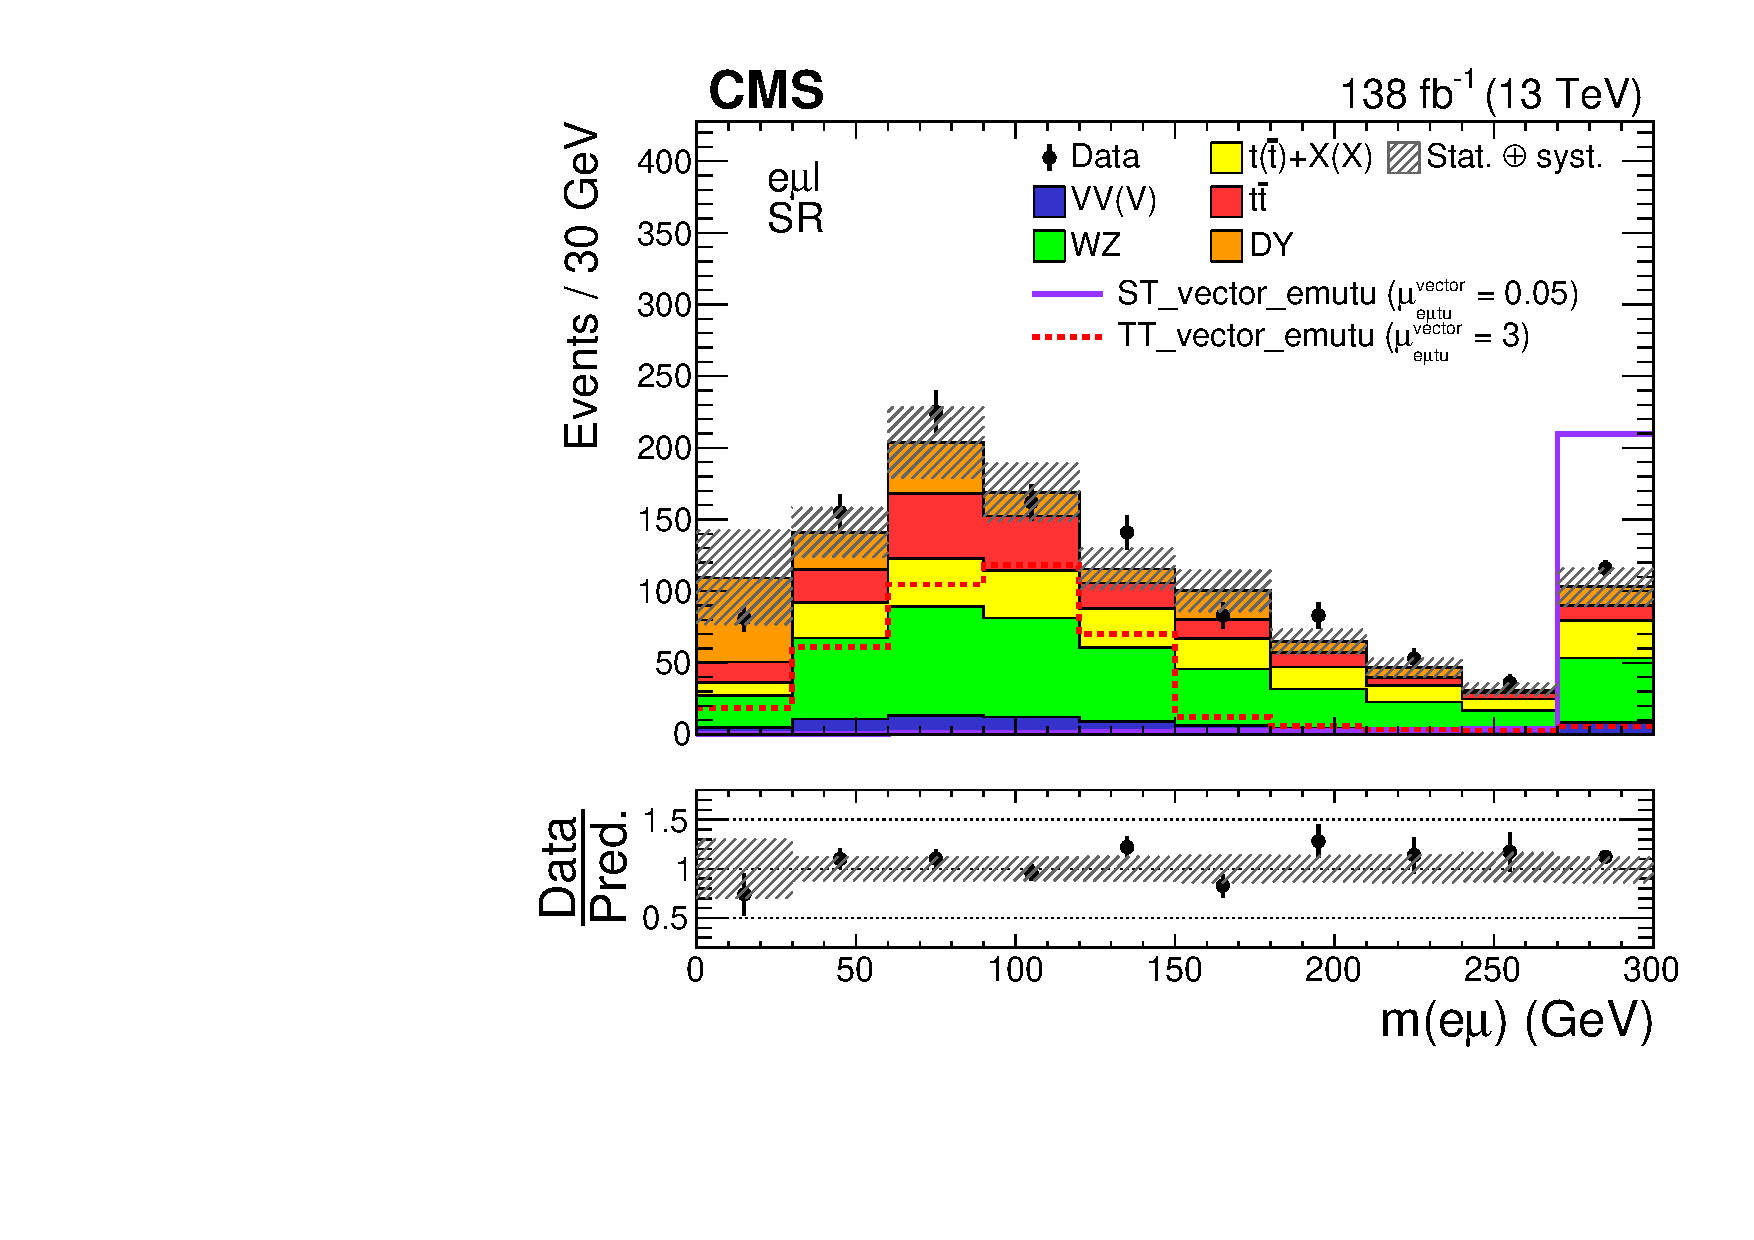
\includegraphics[width=0.45\textwidth]{figures/Part3/Selection/Memu}&
 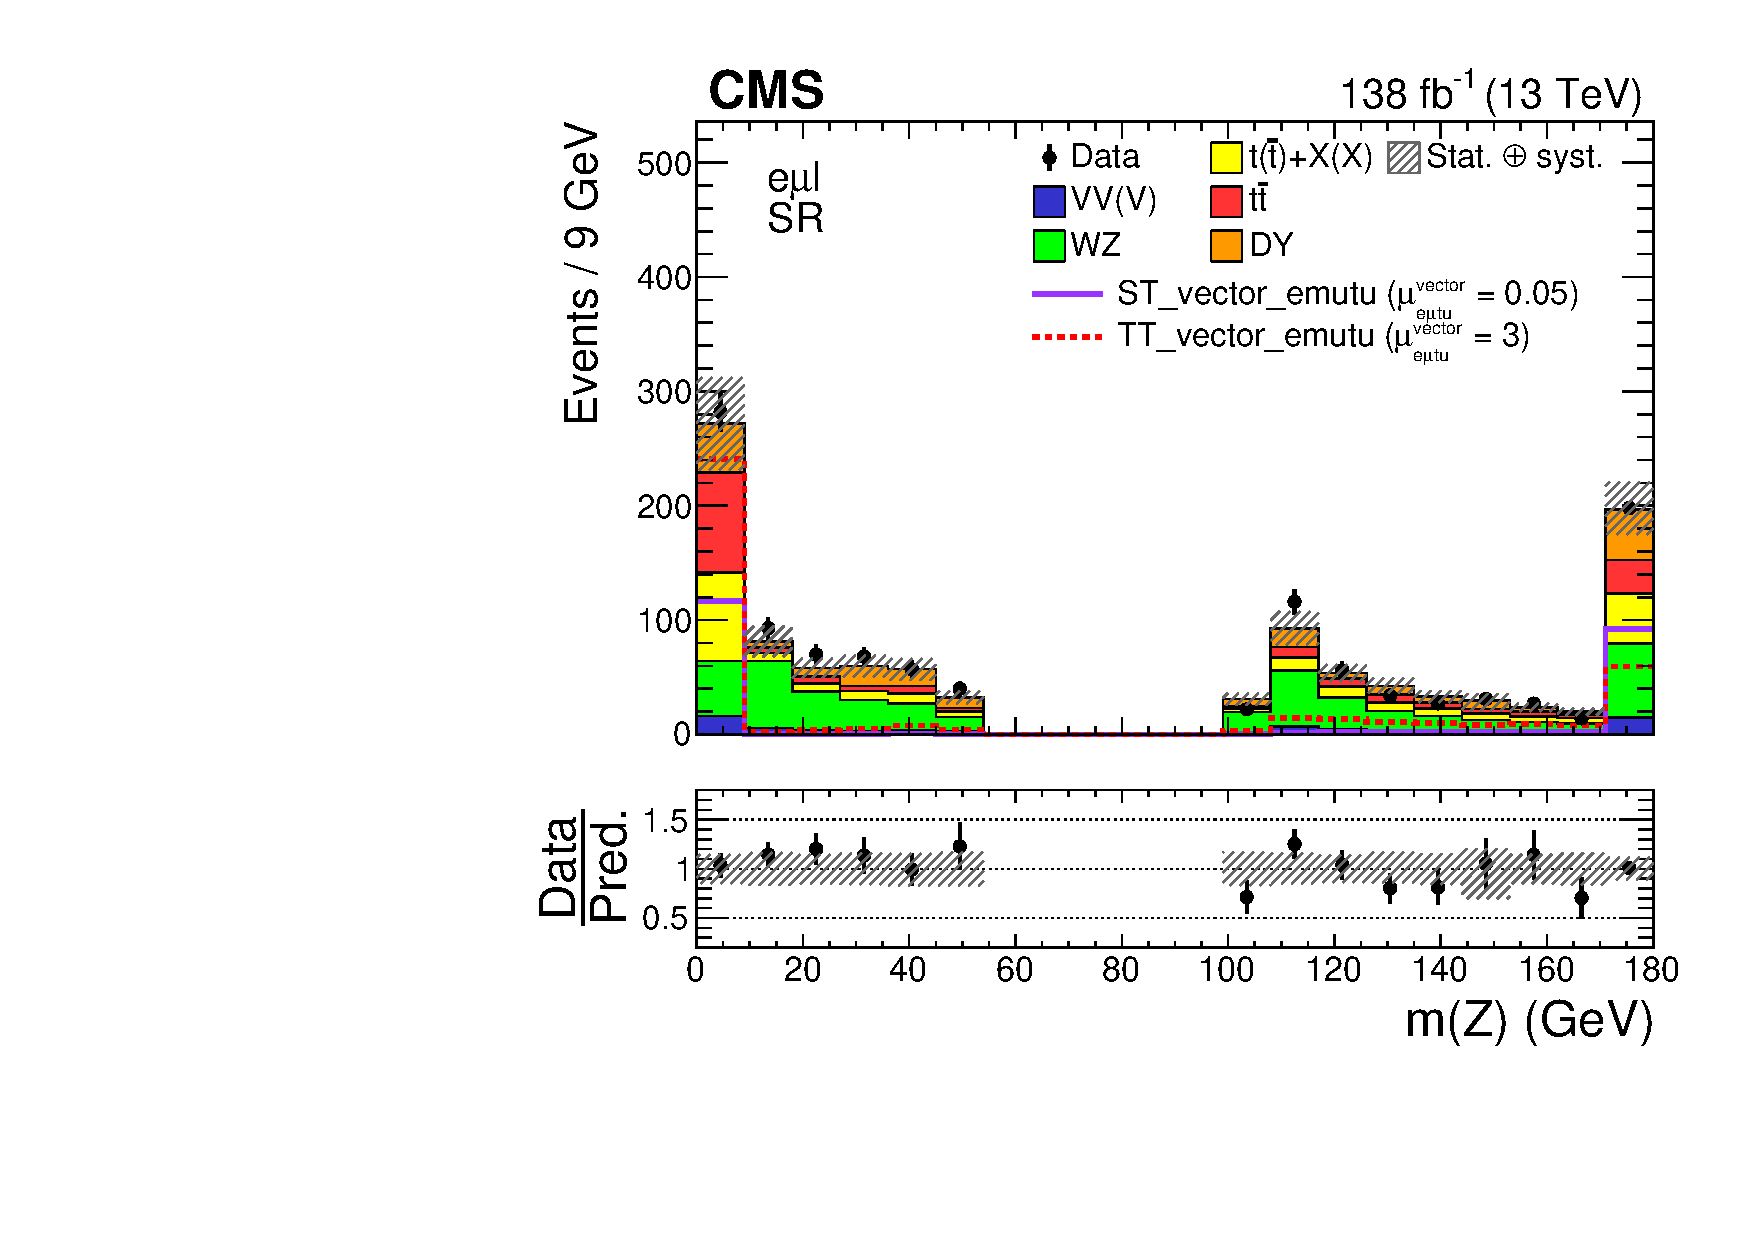
\includegraphics[width=0.45\textwidth]{figures/Part3/Selection/Zmass} \\
 \end{tabular}
 \caption{Distributions of the LFV e$\upmu$ mass (left) and the Z boson mass (right) in \ac{SR}. The data are shown as filled points and the \ac{SM} background predictions as histograms. The VV(V) background includes ZZ and triboson production, while the $\ttbar$ + X(X) component includes $\ttbar$W, $\ttbar$Z, $\ttbar$H, tZq, and smaller backgrounds containing one or two top quarks plus a boson or quark. All backgrounds are estimated using \ac{MC} simulation. The hatched bands indicate statistical and systematic uncertainties for the \ac{SM} background predictions. The normalization of the signal processes is chosen arbitrarily for improved visualization. The last bin of both histograms includes the overflow events.}
 \label{fig:SR}
 \end{center}
\end{figure}

Using the LFV e$\upmu$ mass, the \ac{SR} is further divided into two subsets to create top production and decay enriched regions:

\begin{itemize}
\item SR1, $\textsf{m}(\textsf{e}\upmu)~<$ 150 GeV: top quark decay enriched.
\item SR2, $\textsf{m}(\textsf{e}\upmu)~>$ 150 GeV: top quark production enriched.
\end{itemize}
%%%%%%%%%%%%%%%%%%%%%%%%%%%%%%%%%%%%%%%%%%%%%%%%%%%%%%%%%%%%%
%%%%%%%%%%%%%%%%%%%%%%%%%%%%%%%%%%%%%%%%%%%%%%%%%%%%%%%%%%%%%
\section{Validation Region}
\label{sec:VR}

\begin{figure}[tbh!]
 \begin{center}
 \begin{tabular}{c}
 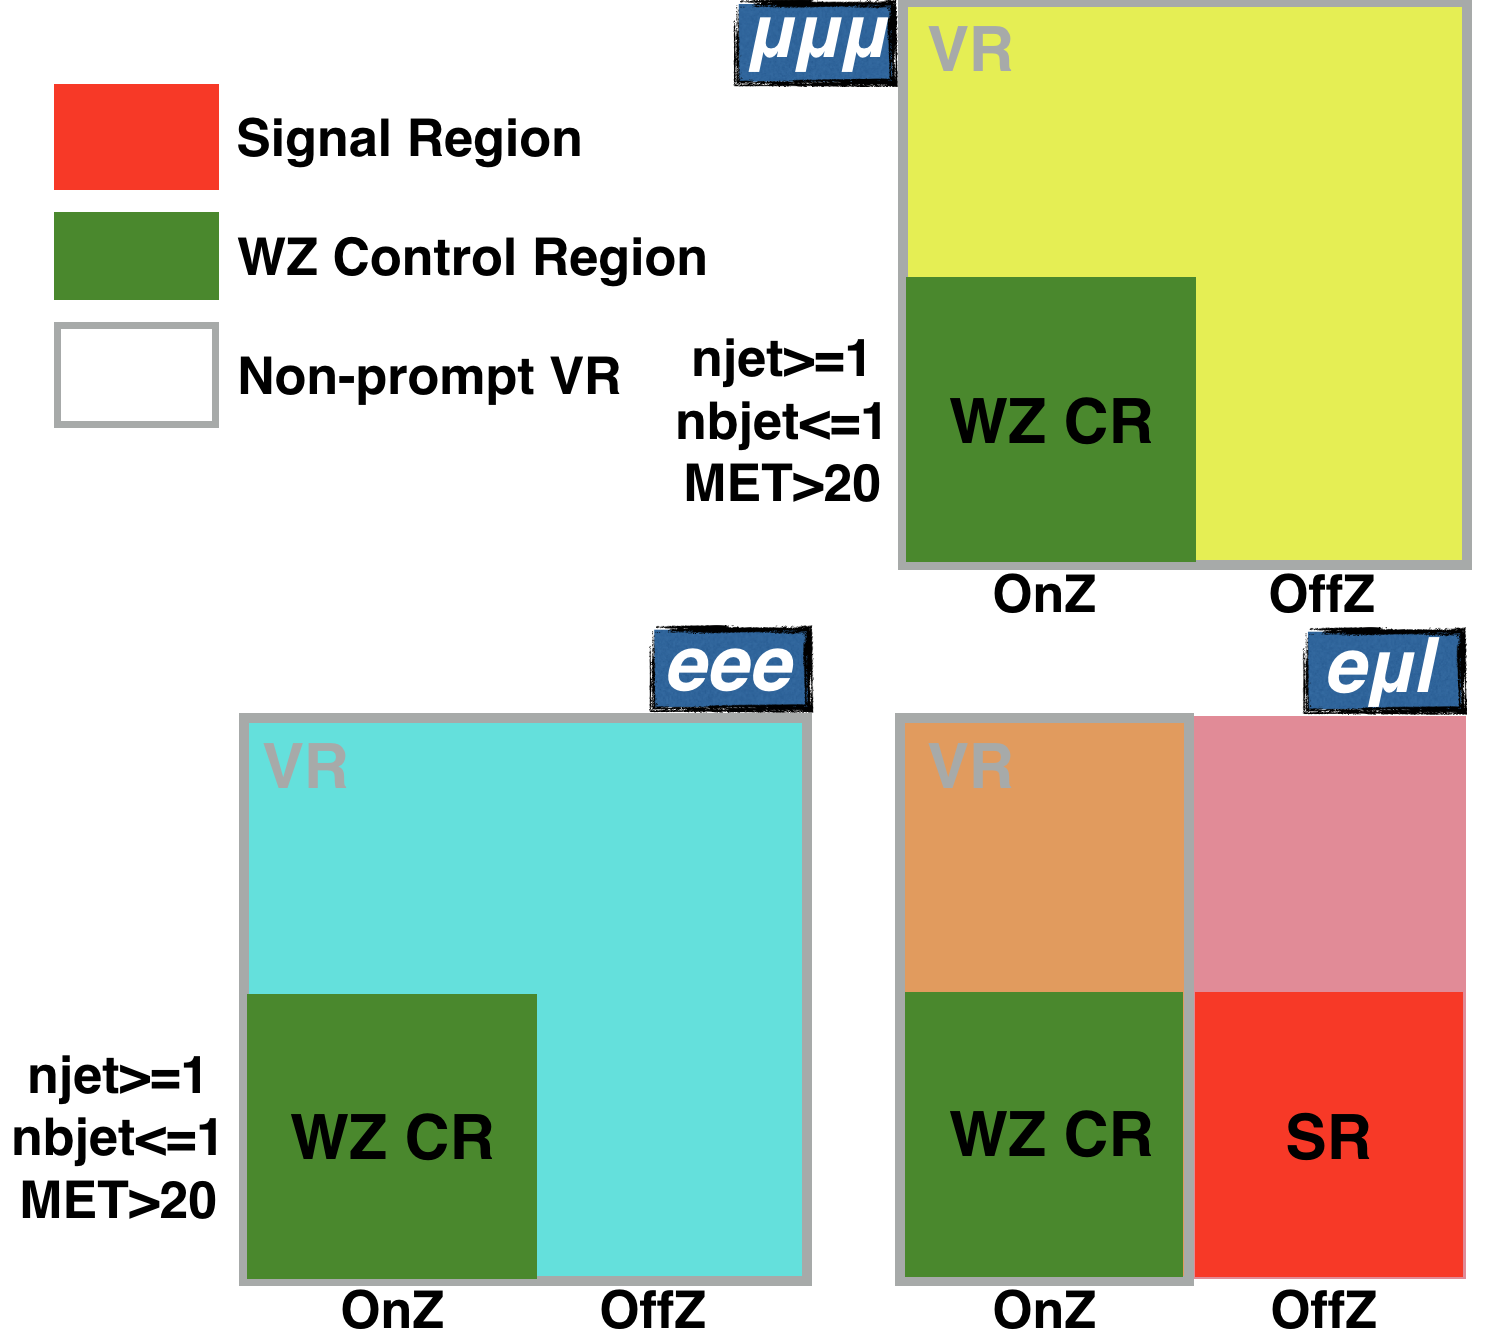
\includegraphics[width=0.8\textwidth]{figures/Part3/Selection/Event}
 \end{tabular}
 \caption{Illustration of selection criteria used to define different regions. ``OnZ'' means the presence of at least one \ac{OSSF} pair with an invariant mass between 50 GeV and 106 GeV. Events are labeled as ``OffZ'' when they fail ``OnZ'' criteria.}
 \label{fig:Event}
 \end{center}
\end{figure}

There are two types of signal-depleted \ac{VR} defined across three channels: \emph{nonprompt} \ac{VR} and WZ \ac{VR}. The purpose of these two types of \ac{VR} is only limited to the validation of the background modeling as neither of them enters the final fit. It is expected that the \emph{nonprompt} \ac{VR} has a significant fraction of \emph{nonprompt} background while WZ production is responsible for most of the backgrounds in the WZ \ac{VR}. Distributions of leading lepton $\pt$ and leading lepton $\eta$ in the WZ control region can be found in Figure~\ref{fig:WZ}. The \emph{nonprompt} \acp{VR} are further discussed in \autoref{chap:Nonprompt}.

Selection criteria used to define different regions are illustrated in Figure~\ref{fig:Event} and are summarized in Table~\ref{tab:region}.

\begin{figure}[tbh!]
 \begin{center}
 \begin{tabular}{cc}
 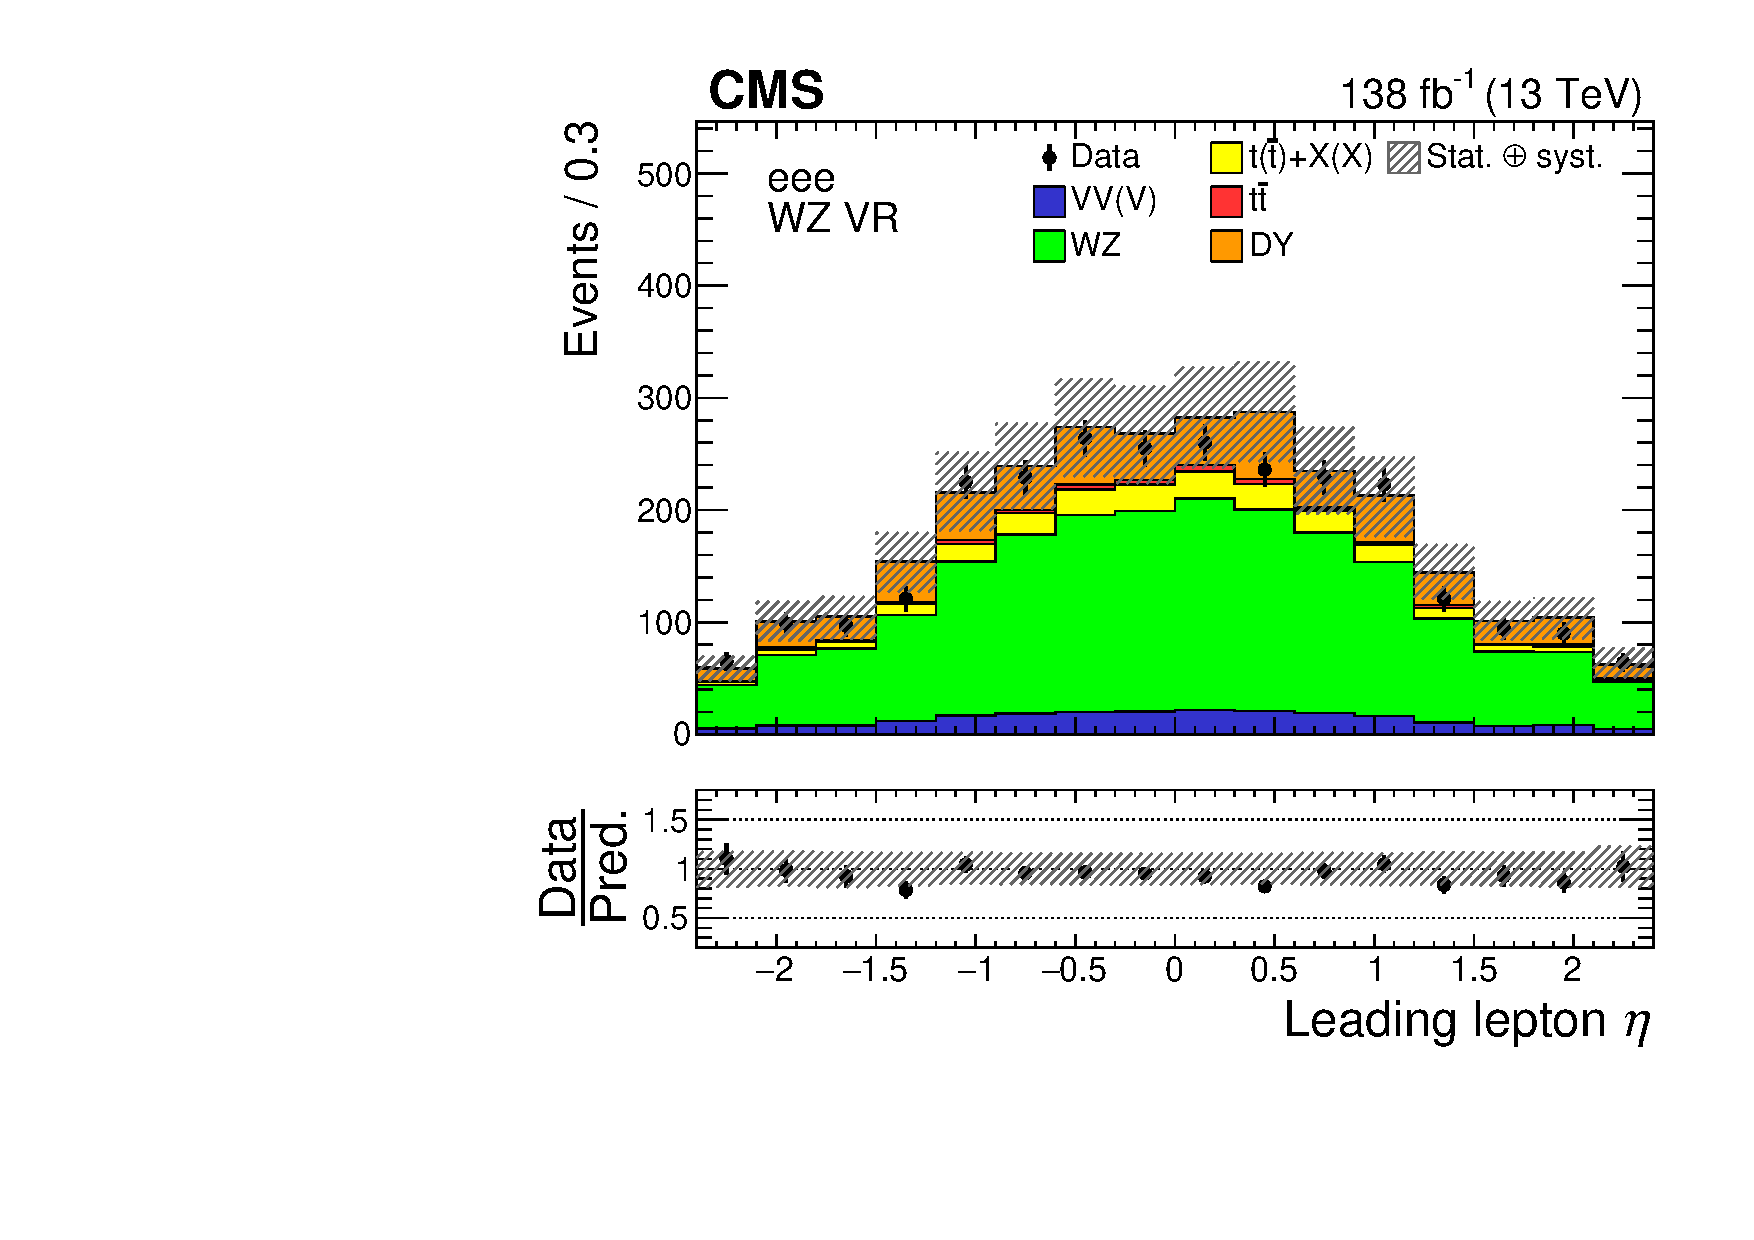
\includegraphics[width=0.45\textwidth]{figures/Part3/Selection/WZ/eee/lep1Eta}&
 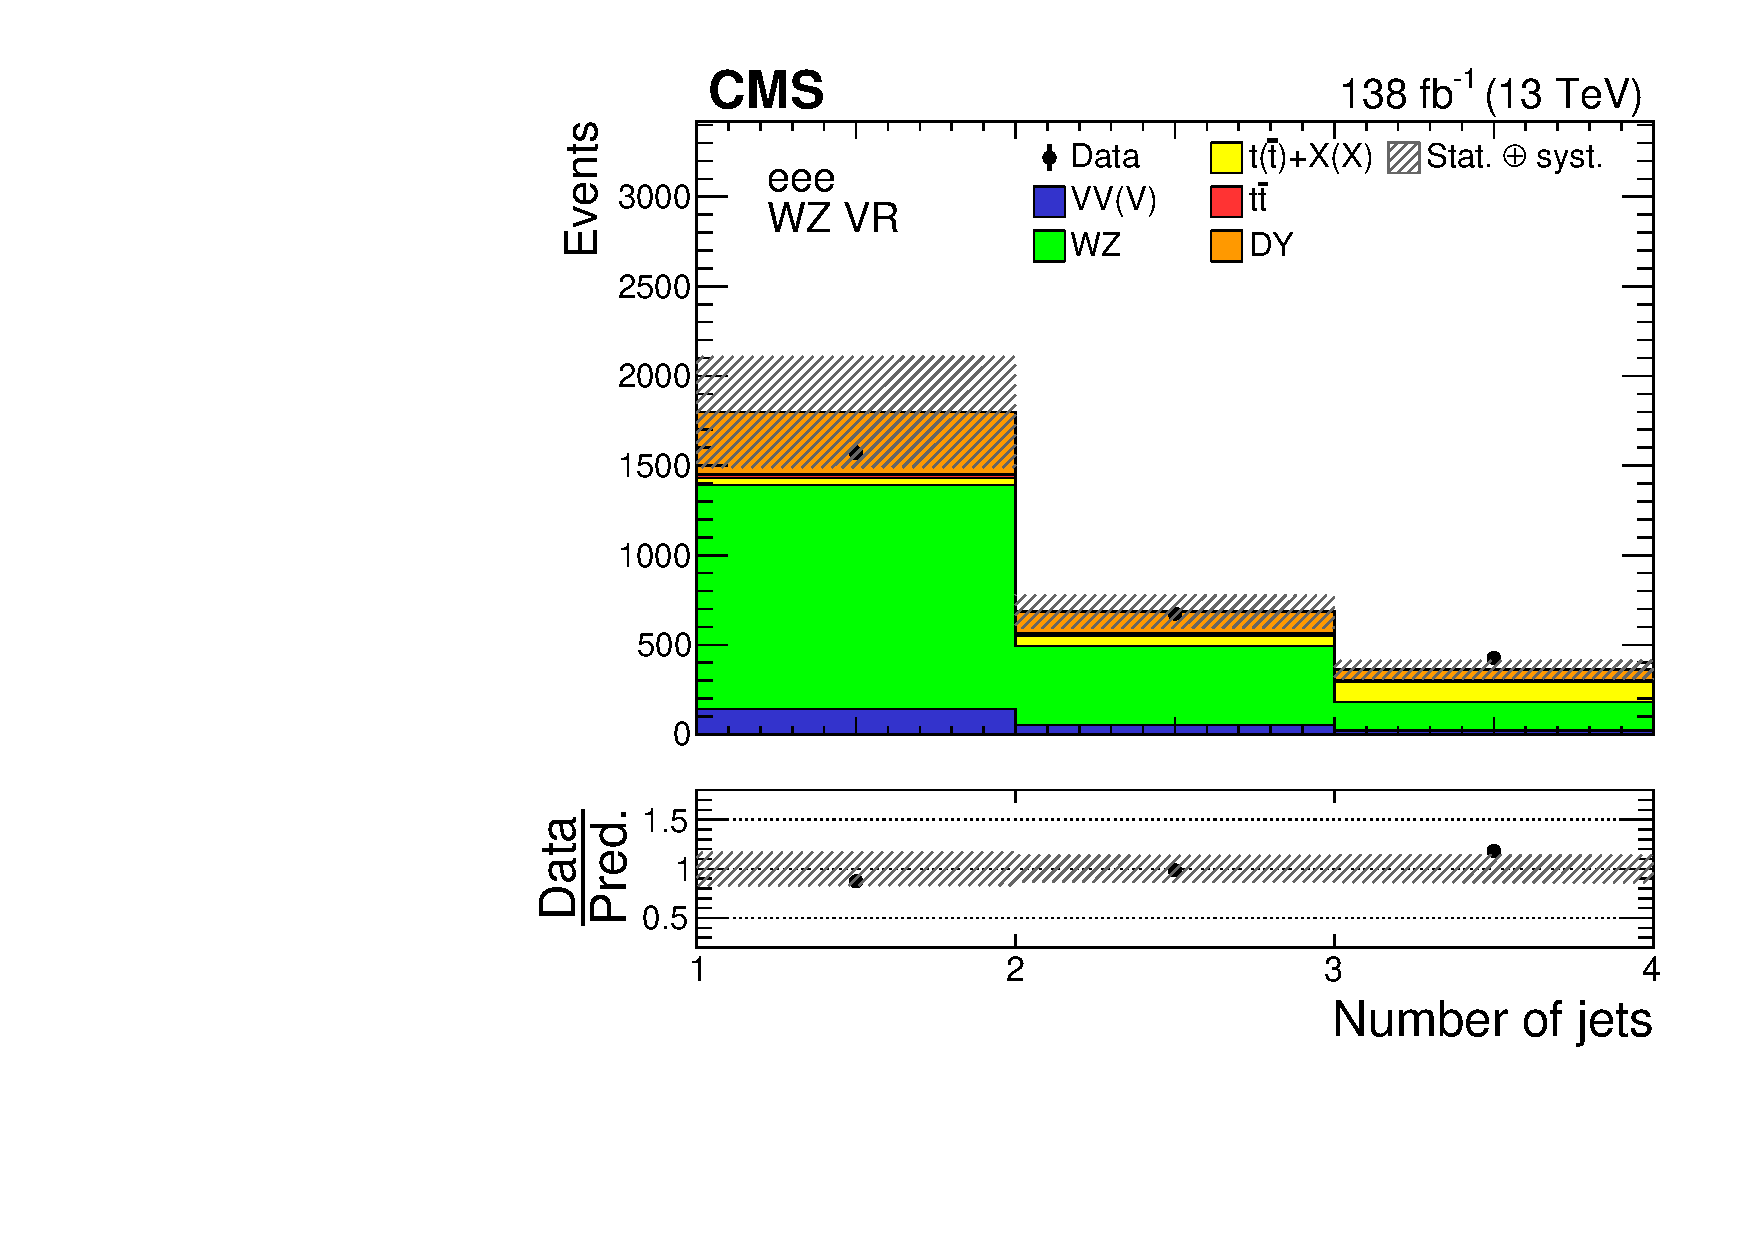
\includegraphics[width=0.45\textwidth]{figures/Part3/Selection/WZ/eee/njet} \\
 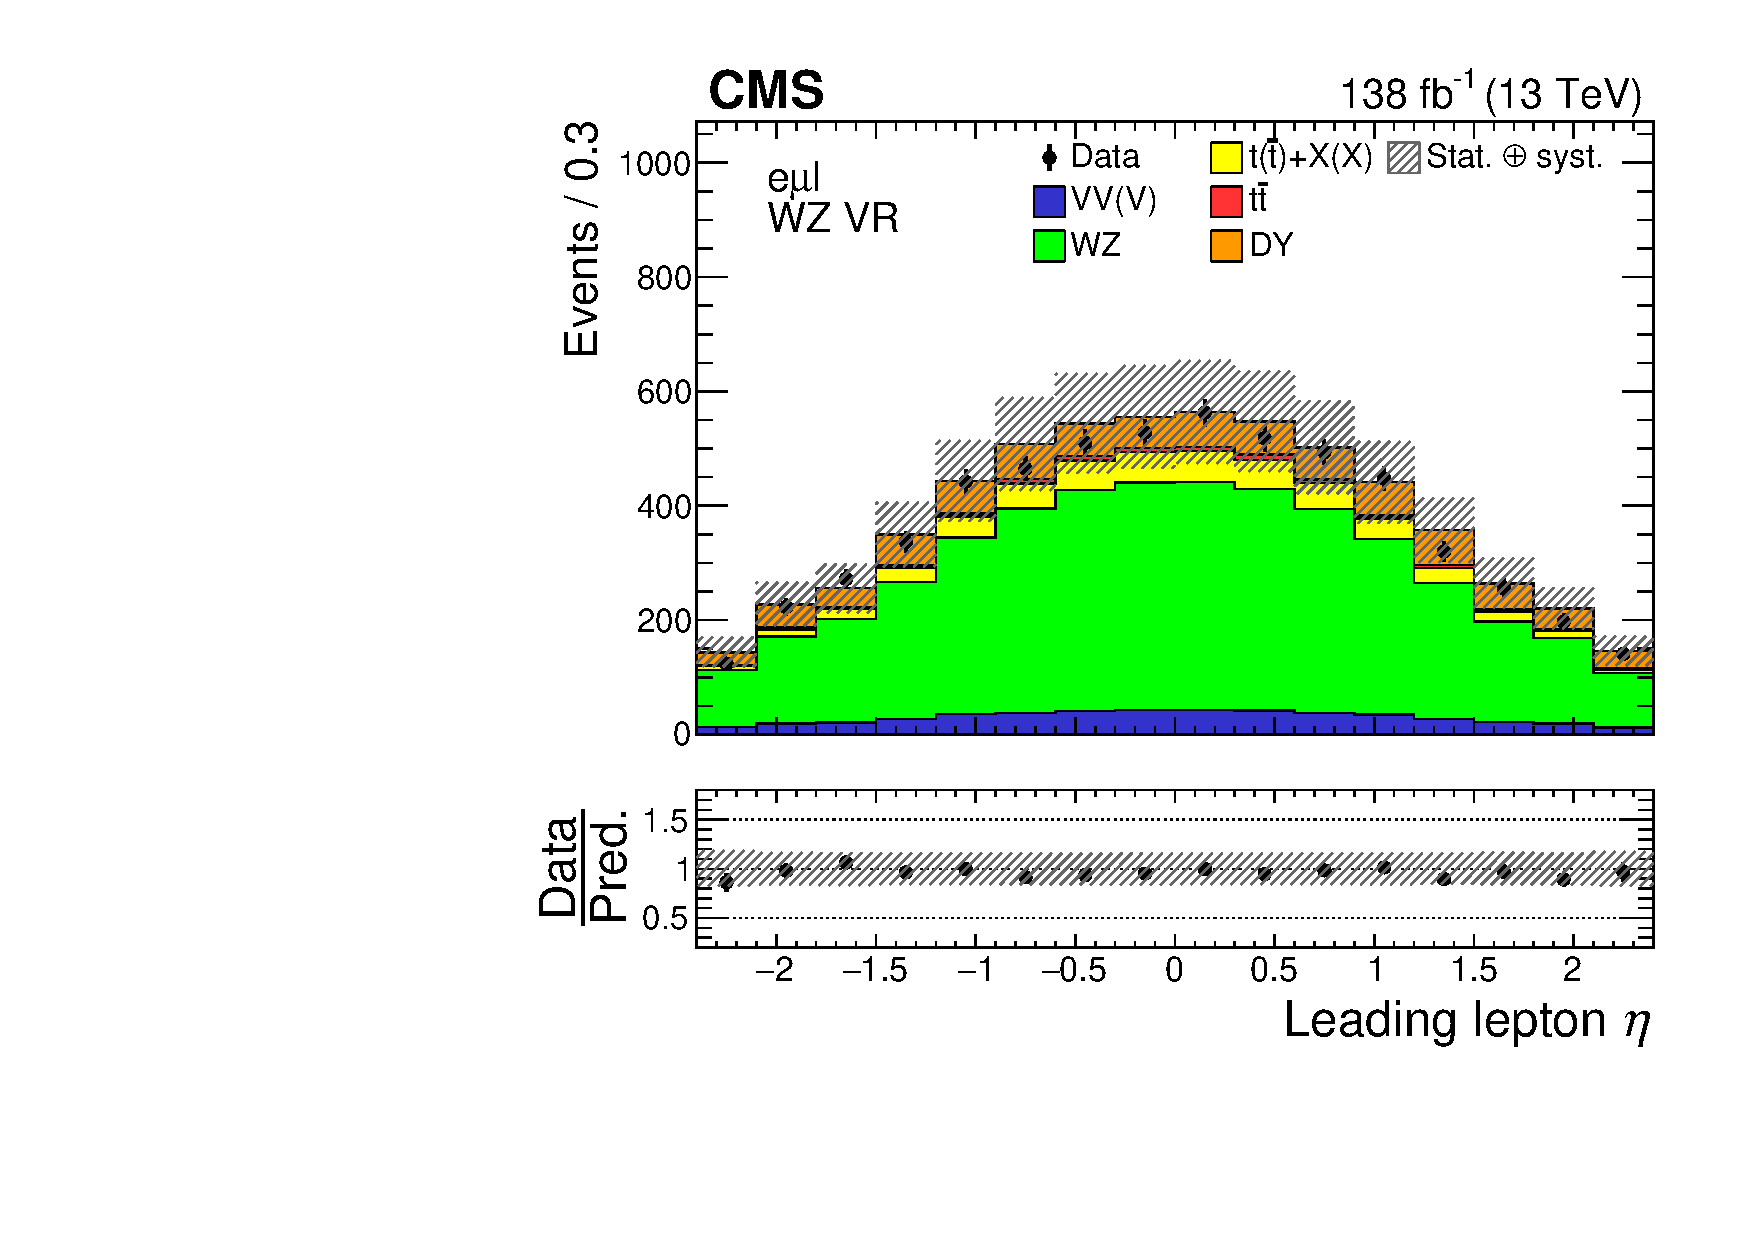
\includegraphics[width=0.45\textwidth]{figures/Part3/Selection/WZ/emul/lep1Eta}&
 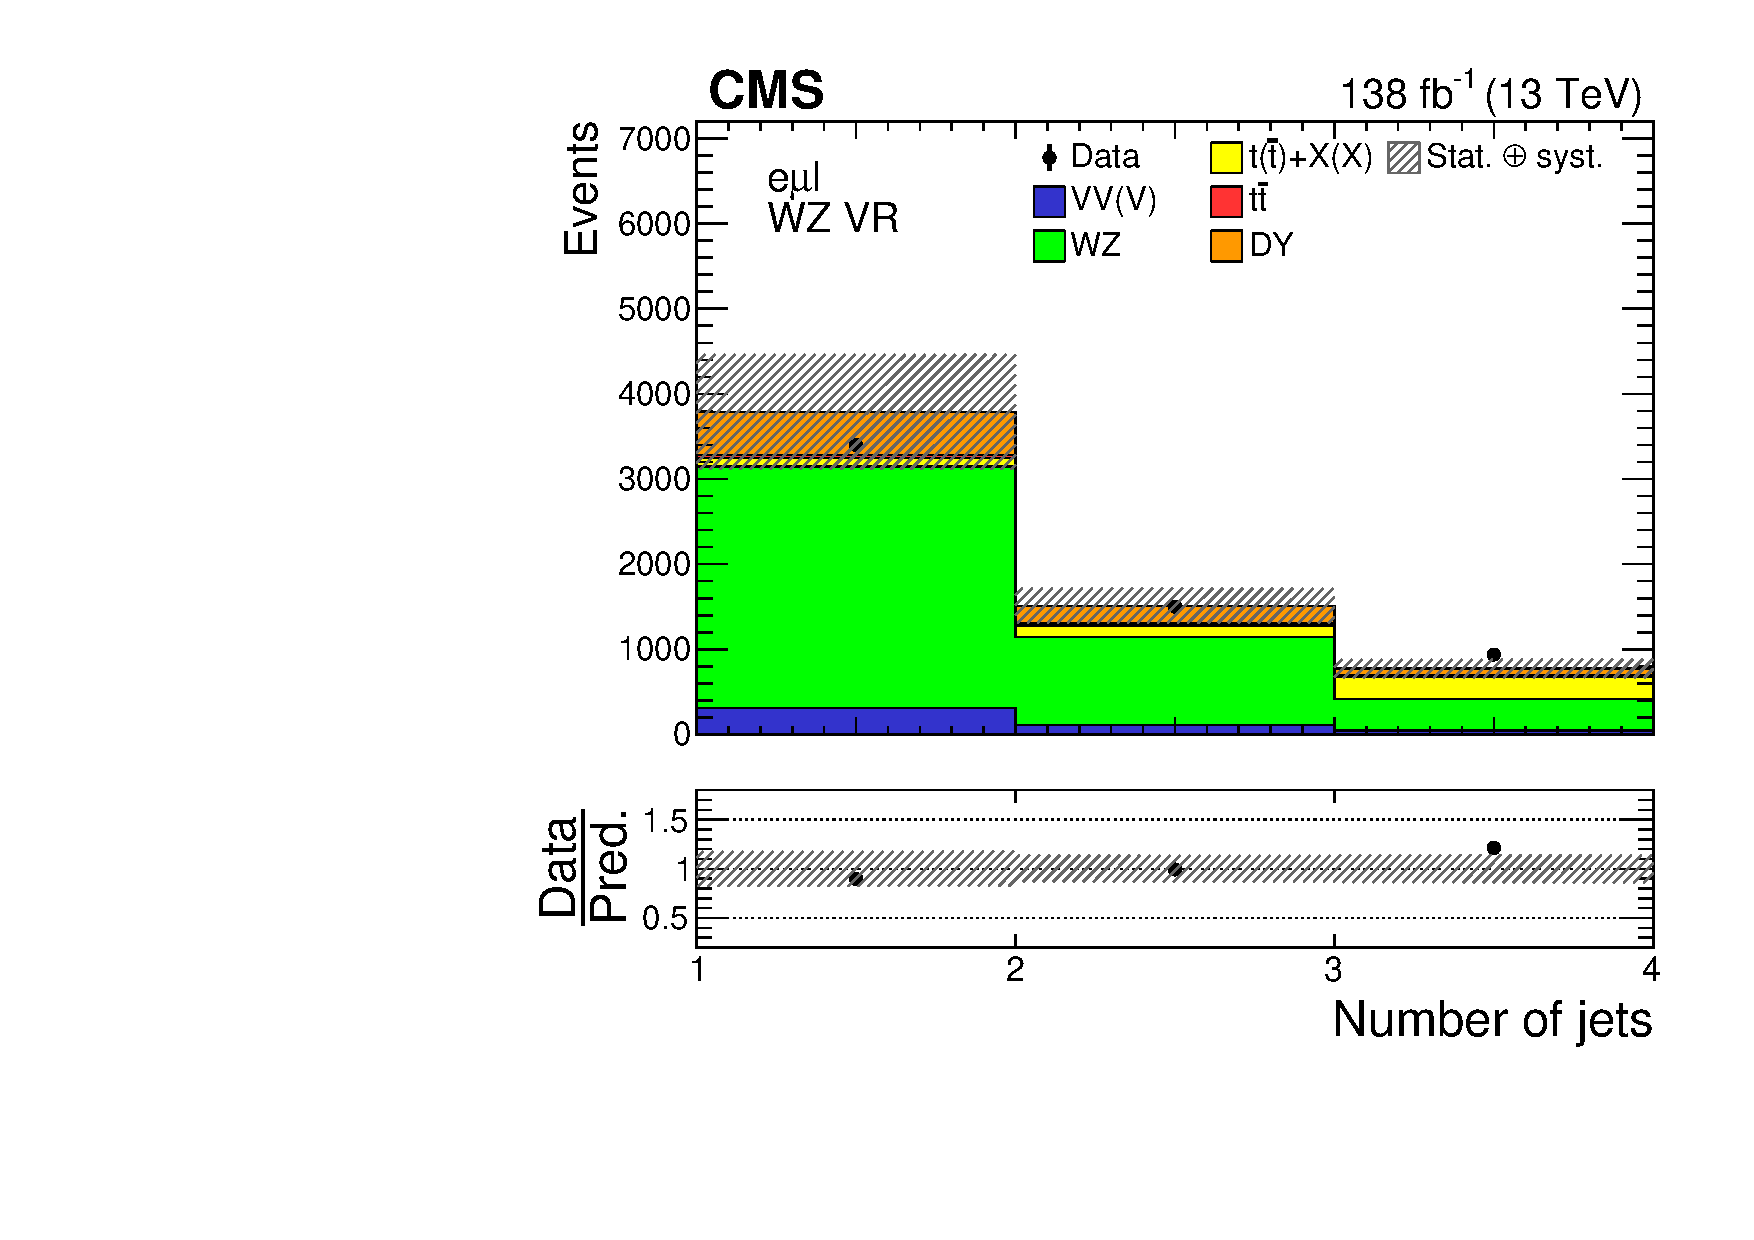
\includegraphics[width=0.45\textwidth]{figures/Part3/Selection/WZ/emul/njet} \\
 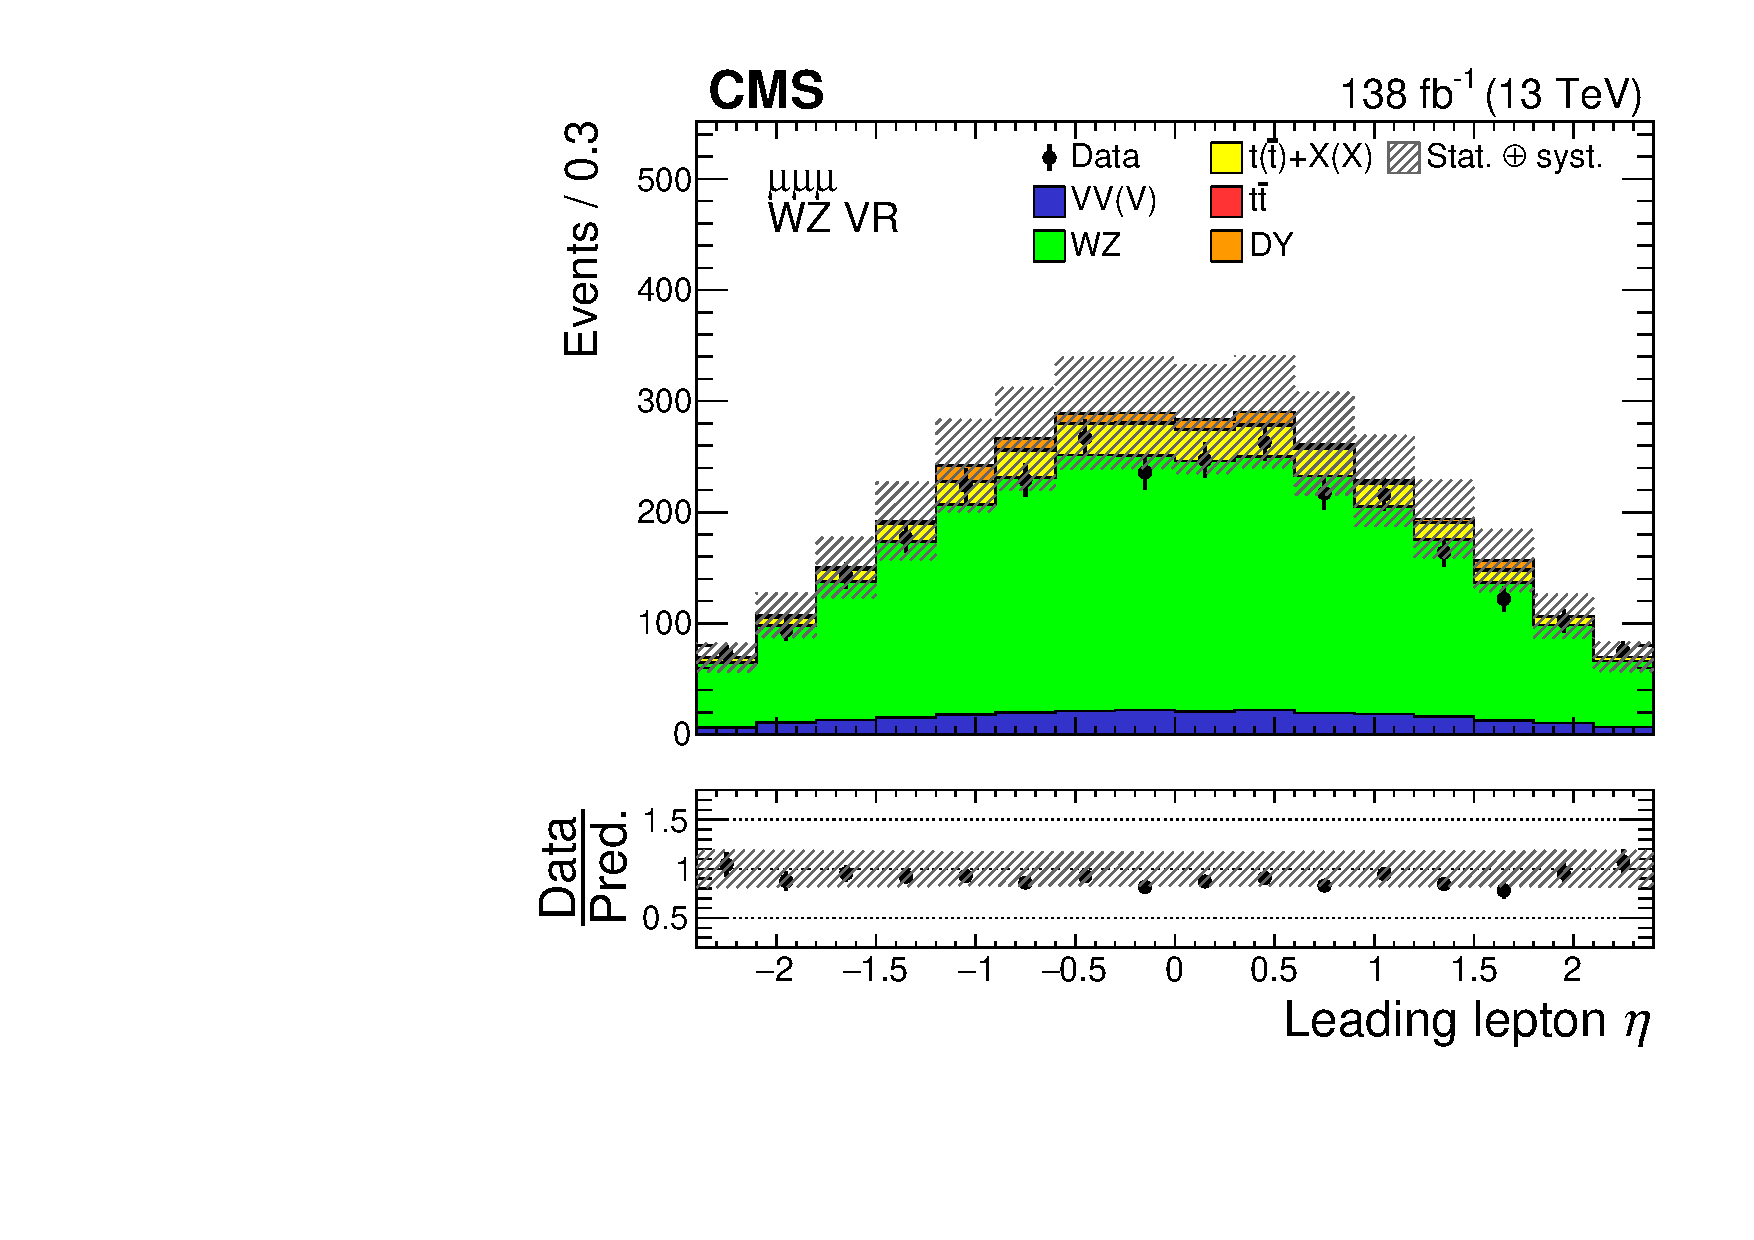
\includegraphics[width=0.45\textwidth]{figures/Part3/Selection/WZ/mumumu/lep1Eta}&
 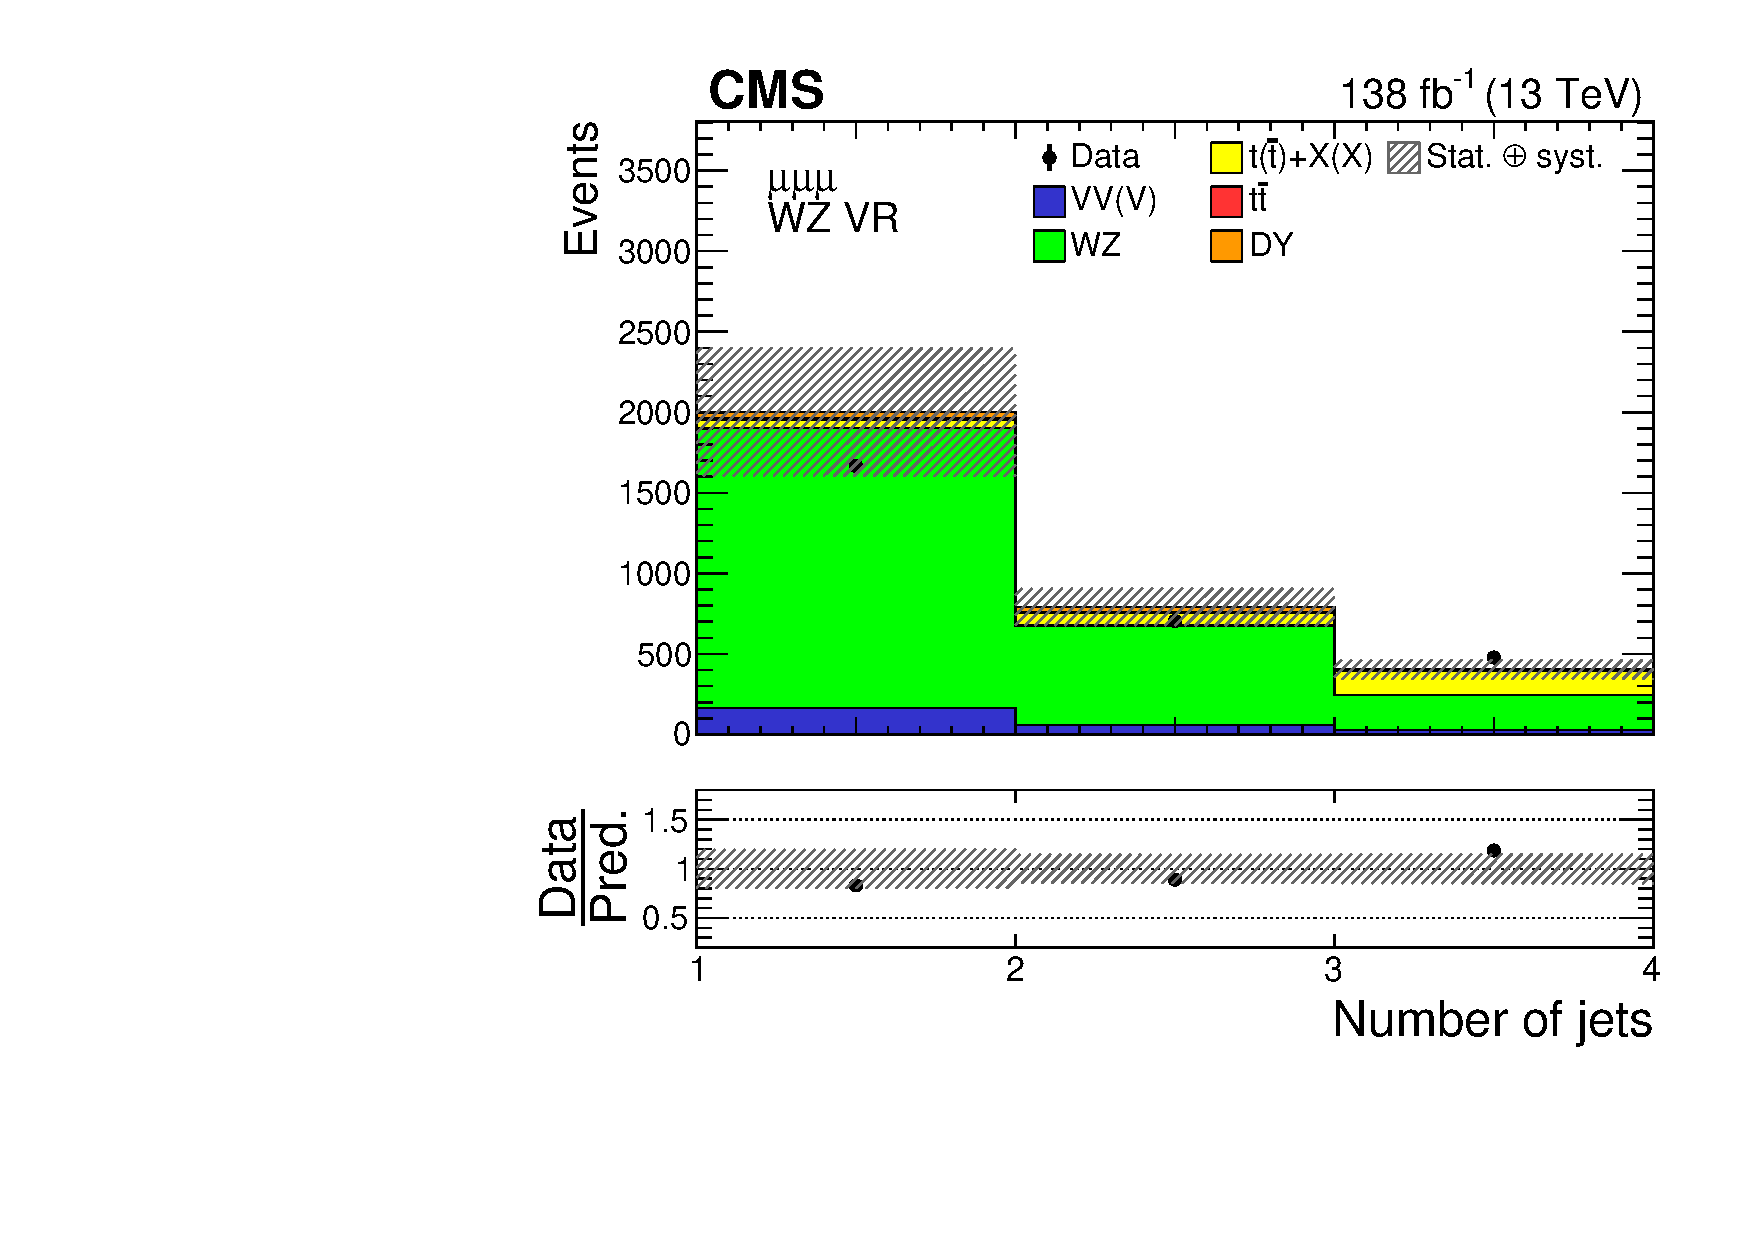
\includegraphics[width=0.45\textwidth]{figures/Part3/Selection/WZ/mumumu/njet} \\
 \end{tabular}
 \caption{Distributions of the leading lepton $\eta$ (left column) and the jet multiplicity (right column) in the WZ \acp{VR}. Events in the eee, $\emul$, and $\mmm$ WZ \acp{VR} are shown in the upper, middle, and lower row, respectively. The data are shown as filled points and the background predictions as histograms. All backgrounds are estimated with \ac{MC} simulation. The hatched bands indicate statistical and systematic uncertainties for the background predictions. The last bin of the right column histograms includes the overflow events.}
 \label{fig:WZ}
 \end{center}
\end{figure}

\begin{table}[th]
\sffamily
\centering
\caption{Summary of the selection criteria used to define different event regions. ``OnZ'' means the presence of at least one \ac{OSSF} pair with an invariant mass between 50 GeV and 106 GeV. Events are labeled as ``OffZ'' when they fail ``OnZ'' criteria.}
\begin{tabular}{cccccccc}
\toprule
Channel     &Region & OnZ & OffZ & MET $>$ 20 GeV &njet$>=$1 &nbjet$<=$1\\ \midrule
\multirow{2}{*}{eee}   & VR & -    & -    & -    & -   & -  \\  
      & WZ VR & \checkmark  & -    & \checkmark  & \checkmark & \checkmark\\ \midrule
\multirow{3}{*}{e$\upmu\ell$}  & SR  & -    & \checkmark  & \checkmark  & \checkmark & \checkmark \\
      & Nonprompt VR  & \checkmark  & -    & -    & -   & -   \\
      & WZ VR & \checkmark  & -    & \checkmark  & \checkmark & \checkmark \\ \midrule
\multirow{2}{*}{$\upmu\upmu\upmu$} & Nonprompt VR  & -    & -    & -    & -   & -   \\  
      & WZ VR & -    & \checkmark  & \checkmark & \checkmark & \checkmark \\ \bottomrule  
\end{tabular}
\label{tab:region}
\end{table}
%%%%%%%%%%%%%%%%%%%%%%%%%%%%%%%%%%%%%%%%%%%%%%%%%%%%%%%%%%%%%
%%%%%%%%%%%%%%%%%%%%%%%%%%%%%%%%%%%%%%%%%%%%%%%%%%%%%%%%%%%%%
\section{Kinematic Reconstruction}
\label{sec:Kin}

As mentioned, the LFV e$\upmu$ pair is assumed to be the product of the \ac{CLFV} interaction, while the third lepton, referred to as the standalone lepton, is assumed to originate from the leptonically decaying top quark. To distinguish this top quark (t$\rightarrow\ell\nu$b) from the top quark that decays via the \ac{CLFV} interaction (t$\rightarrow\textsf{e}\upmu$q), the former is referred to as the \ac{SM} top quark while the latter is referred to as the LFV top quark. 

Jet with the highest b-tagging score, regardless of whether or not it crosses the medium working point threshold, is assumed to originate from bottom quark decay. Therefore, it is combined with \ac{MET} to build the \ac{SM} top quark. The x and y components of \ac{MET} are taken as measurements of neutrino $p_{\textsf{x}}$ and $p_{\textsf{y}}$. The z component of neutrino momentum is calculated by imposing the constraint that the invariant mass of the combined object (standalone lepton + neutrino) must be equal to W boson mass. If there is no real solution, the real part of the complex solution is taken. If there is more than one real solution, the solution that is the closest to the $p_{\textsf{z}}$ of the standalone lepton is taken. In events where there is more than one candidate of standalone lepton (i.e. the presence of the \ac{SSSF} pair), the lepton that gives a top mass that is the closest to the \ac{SM} top quark mass ($\mt$ = 172.5 GeV) is taken as the standalone lepton.

Once the standalone lepton has been determined, the remaining two leptons are labeled as the LFV e$\upmu$ pair and are combined with each selected jet to reconstruct the LFV top quark candidates. Jet with the highest b-tagging score is excluded from this reconstruction since it is assumed to be from the decay of the \ac{SM} top quark. Out of all the LFV top quark candidates, the candidate that gives a top mass that is the closest to the \ac{SM} top quark mass is taken. The LFV top quark mass is set to 0 in events where there are less than two jets.

Z boson candidate is reconstructed using the \ac{OSSF} pair, which is not guaranteed to be present in the $\emul$ channel. The Z boson mass ($\mz$) is set to 0 in events where the \ac{OSSF} is absent. Z boson candidate is the only heavy particle reconstructed in the eee and $\mmm$ channels. Since there are always two ways to form the \ac{OSSF} pair, the \ac{OSSF} pair with an invariant mass that is closer to the Z boson mass ($\mz$ = 91.2 GeV) is taken. 

Jets with high b-tagging scores are combined with leptons to form so-called ``$\mbl$'' systems. The first $\mbl$ system takes the jet with the highest b-tagging score and combines it with each \emph{tight} lepton in events. Out of the three $\mbl$ system candidates, the one with the lowest $\mbl$ is taken, and the two constitutes are excluded from the consideration of the second $\mbl$ system. If additional jets exist, the second $\mbl$ system takes the jet with the highest b-tagging score and combines it with two of the remaining leptons separately. Out of the two candidates, the one with the lowest $\mbl$ is taken. $\mbl$ is set to 0 if no additional jet exists after the formation of the first $\mbl$ system.